\documentclass[a4paper, 12pt]{article}

%%% Работа с русским языком
\usepackage{cmap}					% поиск в PDF
\usepackage{mathtext} 				% русские буквы в формулах
\usepackage[T2A]{fontenc}			% кодировка
\usepackage[utf8]{inputenc}			% кодировка исходного текста
\usepackage[russian]{babel}	% локализация и переносы

%%% Дополнительная работа с математикой
\usepackage{amsmath,amsfonts,amssymb,amsthm,mathtools} % AMS
\usepackage{icomma} % "Умная" запятая: $0,2$ --- число, $0, 2$ --- перечисление

%% Номера формул
%\mathtoolsset{showonlyrefs=true} % Показывать номера только у тех формул, на которые есть \eqref{} в тексте.

%% Шрифты
\usepackage{euscript}	 % Шрифт Евклид
\usepackage{mathrsfs} % Красивый матшрифт

%% Поля
\usepackage[left=2cm,right=2cm,top=2cm,bottom=2cm,bindingoffset=0cm]{geometry}

%% Русские списки
\usepackage{enumitem}
\makeatletter
\AddEnumerateCounter{\asbuk}{\russian@alph}{щ}
\makeatother

%%% Работа с картинками
\usepackage{graphicx}  % Для вставки рисунков
\graphicspath{{images/}{images2/}}  % папки с картинками
\setlength\fboxsep{3pt} % Отступ рамки \fbox{} от рисунка
\setlength\fboxrule{1pt} % Толщина линий рамки \fbox{}
\usepackage{wrapfig} % Обтекание рисунков и таблиц текстом

%%% Работа с таблицами
\usepackage{array,tabularx,tabulary,booktabs} % Дополнительная работа с таблицами
\usepackage{longtable}  % Длинные таблицы
\usepackage{multirow} % Слияние строк в таблице

%% Красная строка
\setlength{\parindent}{2em}

%% Интервалы
\linespread{1}
\usepackage{multirow}

%% TikZ
\usepackage{tikz}
\usetikzlibrary{graphs,graphs.standard}

%% Верхний колонтитул
\usepackage{fancyhdr}
\pagestyle{fancy}

%% Перенос знаков в формулах (по Львовскому)
\newcommand*{\hm}[1]{#1\nobreak\discretionary{}
	{\hbox{$\mathsurround=0pt #1$}}{}}

%% Мои дополнения
\usepackage{float} %Добавляет возможность работы с командой [H] которая улучшает расположение на странице
\usepackage{gensymb} %Красивые градусы
\usepackage{graphicx}               % Импорт изображений
\usepackage{caption} % Пакет для подписей к рисункам, в частности, для работы caption*

% подключаем hyperref (для ссылок внутри  pdf)
\usepackage[unicode, pdftex]{hyperref}

%%% Теоремы
\theoremstyle{plain}                    % Это стиль по умолчанию, его можно не переопределять.
\renewcommand\qedsymbol{$\blacksquare$} % переопределение символа завершения доказательства

\newtheorem{theorem}{Теорема}[section] % Теорема (счетчик по секиям)
\newtheorem{proposition}{Утверждение}[section] % Утверждение (счетчик по секиям)
\newtheorem{definition}{Определение}[section] % Определение (счетчик по секиям)
\newtheorem{corollary}{Следствие}[theorem] % Следстиве (счетчик по теоремам)
\newtheorem{problem}{Задача}[section] % Задача (счетчик по секиям)
\newtheorem*{remark}{Примечание} % Примечание (можно переопределить, как Замечание)
\newtheorem{lemma}{Лемма}[section] % Лемма (счетчик по секиям)

\begin{document}
	\newcommand{\HRule}{\rule{\linewidth}{0.7mm}} % Defines a new command for the horizontal lines, change thickness here
	
	\begin{center}
		\large\textbf{Московский Физико-Технический Институт}\\ % Name of your university/college
		\large\textbf{(государственный университет)}
	
		\vfill
		
		\Large Лабораторная работа по курсу общей физики № *labnum*\\[0.5cm] % Preambule of your document title
		
		
		\HRule
		\\[0.4cm]
		{ \huge \bfseries *name of your labwork*}% Title of your document
		\\[0.4cm] 
		\HRule
		\\[0.5cm]
		
		\ \\
	\textbf{\large Автор:} \\	
	\large *your name* *groupname*\\ % Your name and something more, your group num for example
		\vfill
		\hspace*{-0.8 cm}
\includegraphics[width=100 pt]{frkt_logo}\\ % logo of your  company/university/college
		\large Долгопрудный, 2021 % location and year
	\end{center}

\newpage
\setcounter{page}{2}
\fancyfoot[c]{\thepage}
\fancyhead[L] {Работа № *labnum*} % some information in page header
\fancyhead[R]{}


	\paragraph*{Цель работы:} 
	\begin{itemize}
		\item При помощи модели абсолютно чёрного тела проведение измерения температуры оптическим пирометром с исчезающей нитью и термопарой
		\item Определение постоянных Планка и Стефана-Больцмана
	\end{itemize}

	\paragraph*{В работе используются:}
	\begin{itemize}
		\item оптический пирометр
		\item модель абсолютно чёрного тела
		\item вольфрамовая лампа
		\item неоновая лампа
		\item блок питания
		\item цифровые вольтметр и амперметр
		\item термопара
	\end{itemize}

	\section*{Теоретическая часть}

	Для измерения температуры разогретых тел, удалённых от наблюдателя, применяют методы оптической пирометрии, основанные на использовании зависимости испускательной способности исследуемого тела от температуры. Различают три температуры, функционально связанные с истинной термодинамической температурой и излучательной способностью тела: радиационную $T_{rad}$, цветовую $T_{col}$ и яркостную $T_{br}$. \par
	В работе измеряется яркостная температура. \textbf{Яркостная температура} - это температура абсолютно чёрного тела, при которой его спектральная испускательная способность равна спектральной испускательной способности исследуемого тела при той же длине волны.
	Измерение яркостной температуры раскалённого тела производится при помощи оптического пирометра с исчезающей нитью, основанного на визуальном сравнении яркости раскалённой нити с яркостью изображения исследуемого тела. \par
	Яркостная температура тела всегда ниже его термодинамической температуры. Это связано с тем, что любое нечёрное тело излучает меньше, чем АЧТ при той же температуре. Зависимость между яркостной и термодинамической температурами вольфрама приведена на рис. \ref{fig:vac}

	\begin{figure}[h]
		\centering
		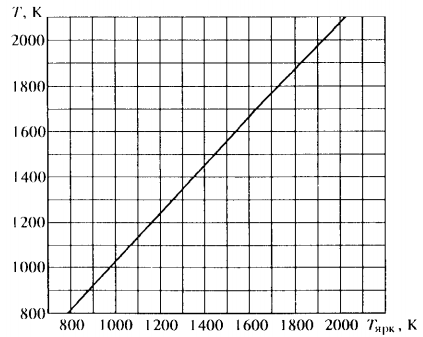
\includegraphics[width=10cm]{Tlight.png}
		\caption{График зависимости $T = f(T_{br})$ для вольфрама}
		\label{fig:vac}
	\end{figure}

	По результатам измерений мощности излучения вольфрамовой нити можно судить о справедливости закона Стефана-Больцмана. Если бы нить излучала как АЧТ, то баланс потребляемой и излучаемой энергии определялся бы соотношением 
	
	\begin{equation} \label{base_equation}
		W = \sigma S (T^4 - T_0^4),
	\end{equation}

	где $W$ - потребляемая нитью электрическая мощность, $S$ - площадь излучающей поверхности нити, $T$ - температура нити, $T_0$ - температура окружающей среды. Однако вольфрамовая нить излучает как серое тел, и излучение её ослаблено по сравнению с АЧТ в $\varepsilon_T$ раз для любой волны при данной температуре тела Т. Тогда предположив, что нить излучает как серое тело и с учётом того, что $T_0 \ll T$, выражение \eqref{base_equation} можно переписать в виде
	
	\begin{equation} \label{2}
		W = \varepsilon_T S \sigma T^4
	\end{equation}

	В справедливости закона Стефана-Больцмана можно убедиться, построив график зависимости $W(T)$ в логарифмическом масштабе и по углу наклона определить показатель степени $n$ исследуемой температурной зависимости. В пределах погрешности показатель степени должен быть близок к четырём. \par
	Также из формулы \eqref{2} можно определить постоянную Стефана-Больцмана.

	\section*{Экспериментальная установка}

	\begin{figure}[h]
		\centering
		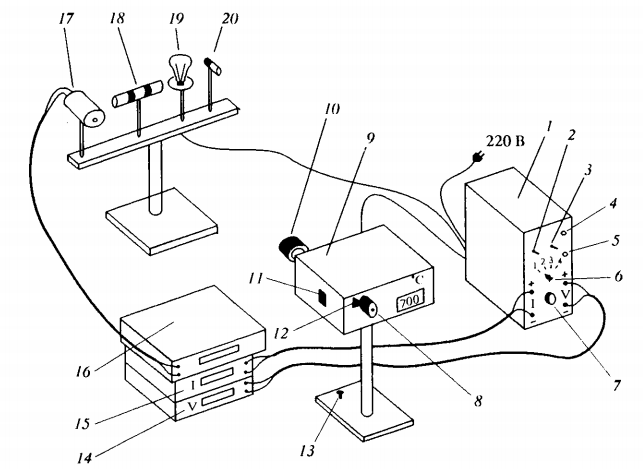
\includegraphics[width=11cm]{scheme.png}
		\caption{Схема экспериментальной установки: 1 - блок питания; 2 - тумблер включения питания образцов; 3 - тумблер нагрева нити пирометра; 4 - кнопка "Нагрев нити"; 5 - кнопка "охлаждение нити"; 6 - тумблер переключения образцов; 7 - регулятор мощности нагрева образцов; 8 - окуляр пирометра; 9 - корпус пирометра; 10 - объектив пирометра; 11 - переключение диапазонов; 12 - ручка смещения красного светофильтра; 13 - регулировочный винт; 14 - вольтметр (напряжение на лампе накаливания); 15 - амперметр (ток через образцы); 16 - вольтметр в цепи термопары; 17 - модель АЧТ; 18 трубка с кольцами из материалов с различной излучательной способностью; 19 - лампа накаливания; 20 - неоновая лампочка}
		\label{fig:scheme}
	\end{figure}

	\section*{Изучение работы оптического пирометра}

	В этом пункте предлагается изучить работу электронного пирометра. Для этого направим пирометр на
	разогретую модель АЧТ и сравним температуры, снятые с помощью термпопары (показатель термопары $k = 41 \text{мкВ/}^oC$) и пирометра.

	\begin{center}
		Температура, полученная с помощью пирометра $T_1 = 1158 ^oC$ \\
		Температура, полученная с помощью термопары $T_2 = 1092 ^oC$ \\
	\end{center}

	Таким образом, получаем, что погрешность определения температуры при помощи пирометра составляется около $6 \%$,
	что не выходит за пределы допустимой нормы.

	\section*{Измерение яркостной температуры накаленных тел}

	\section*{Проверка закона Стефана-Больцмана}

	Направим пирометр на нить лампы накаливания. Постепенно увиличивая температуру, снимем зависимость 
	яркостной температуры от тока и напряжения, подводимых к лампе. Используя эти величины, найдем
	подводимую к лампе мощность, а используя рис. \ref{fig:vac} каждому значению яркостной температуры
	сопоставим значение термодинамической температуры. Результаты запишем в таблицу \ref{table:1}.

	\begin{table}[h!]
    \centering
    \begin{tabular}{|c|c|c|c|c|c|}
    \hline
    $T_{br}$, $^oC$   & $I$, А              & $U$, мВ                & $T$, $^oC$                 & $W$, мВт   & $\varepsilon_W \cdot 10^{-5}$      \\ \hline
    950               & 1,5 $\pm$ 0,1       & 19,84 $\pm$ 0,01       & 962,50   $\pm$ 1           & 29,760     & 51,46                              \\ \hline
    1000              & 1,5 $\pm$ 0,1       & 21,50 $\pm$ 0,01       & 1 016,67 $\pm$ 1           & 32,250     & 47,54                              \\ \hline
    1100              & 1,5 $\pm$ 0,1       & 26,40 $\pm$ 0,01       & 1 125,00 $\pm$ 1           & 39,600     & 38,91                              \\ \hline
    1200              & 1,5 $\pm$ 0,1       & 30,31 $\pm$ 0,01       & 1 233,33 $\pm$ 1           & 45,465     & 33,97                              \\ \hline
    1300              & 1,5 $\pm$ 0,1       & 40,08 $\pm$ 0,01       & 1 341,67 $\pm$ 1           & 60,120     & 26,04                              \\ \hline
    1400              & 1,5 $\pm$ 0,1       & 50,39 $\pm$ 0,01       & 1 450,00 $\pm$ 1           & 75,585     & 21,01                              \\ \hline
    1500              & 1,5 $\pm$ 0,1       & 63,51 $\pm$ 0,01       & 1 558,33 $\pm$ 1           & 95,265     & 17,00                              \\ \hline
    1600              & 1,5 $\pm$ 0,1       & 69,48 $\pm$ 0,01       & 1 666,67 $\pm$ 1           & 104,220    & 15,59                              \\ \hline
    1700              & 1,5 $\pm$ 0,1       & 81,35 $\pm$ 0,01       & 1 775,00 $\pm$ 1           & 122,025    & 13,52                              \\ \hline
    1800              & 1,5 $\pm$ 0,1       & 86,65 $\pm$ 0,01       & 1 883,33 $\pm$ 1           & 129,975    & 12,70                              \\ \hline
    1900              & 1,5 $\pm$ 0,1       & 89,25 $\pm$ 0,01       & 1 991,67 $\pm$ 1           & 133,875    & 12,28                              \\ \hline
    \end{tabular}
    \caption{Эксперементальные данные}
    \label{table:1}
\end{table}

	По измеренным данным построим график зависимости $W = f(T)$.

	\begin{figure}[h]
		\centering
		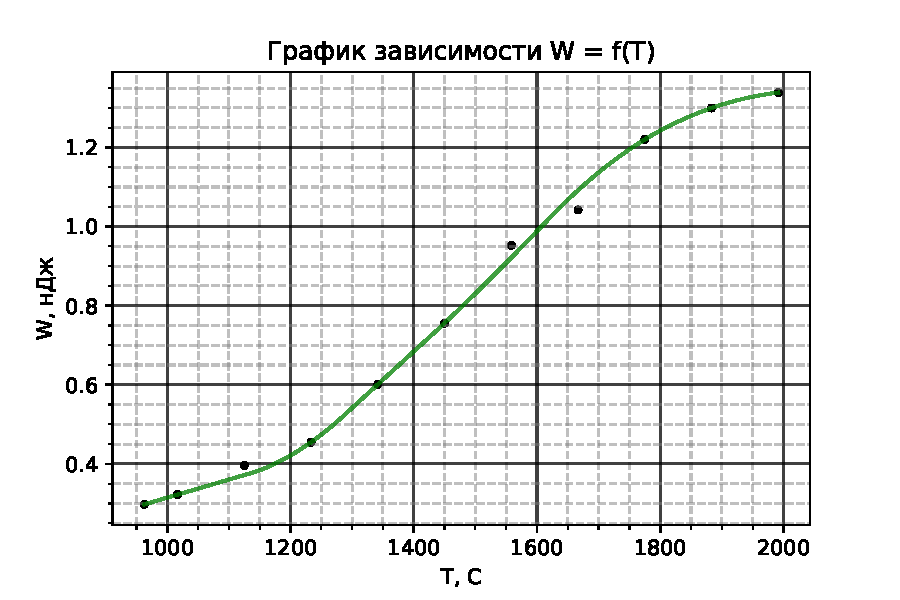
\includegraphics[width=\linewidth]{W.pdf}
		% \caption{}
		\label{fig:W}
	\end{figure}

	Для проверки закона Стефана-Больцмана

	\begin{equation*}
		W = \varepsilon_T B T^n
	\end{equation*}

	построим данный график в логарифмическом масштабе, при этом мы получим функцию

	\begin{equation*}
		\ln W = \ln (\varepsilon_T B) + n \ln T
	\end{equation*}

	после чего сможем опреелить значение $n$ по наклону груфика.

	\begin{figure}[h]
		\centering
		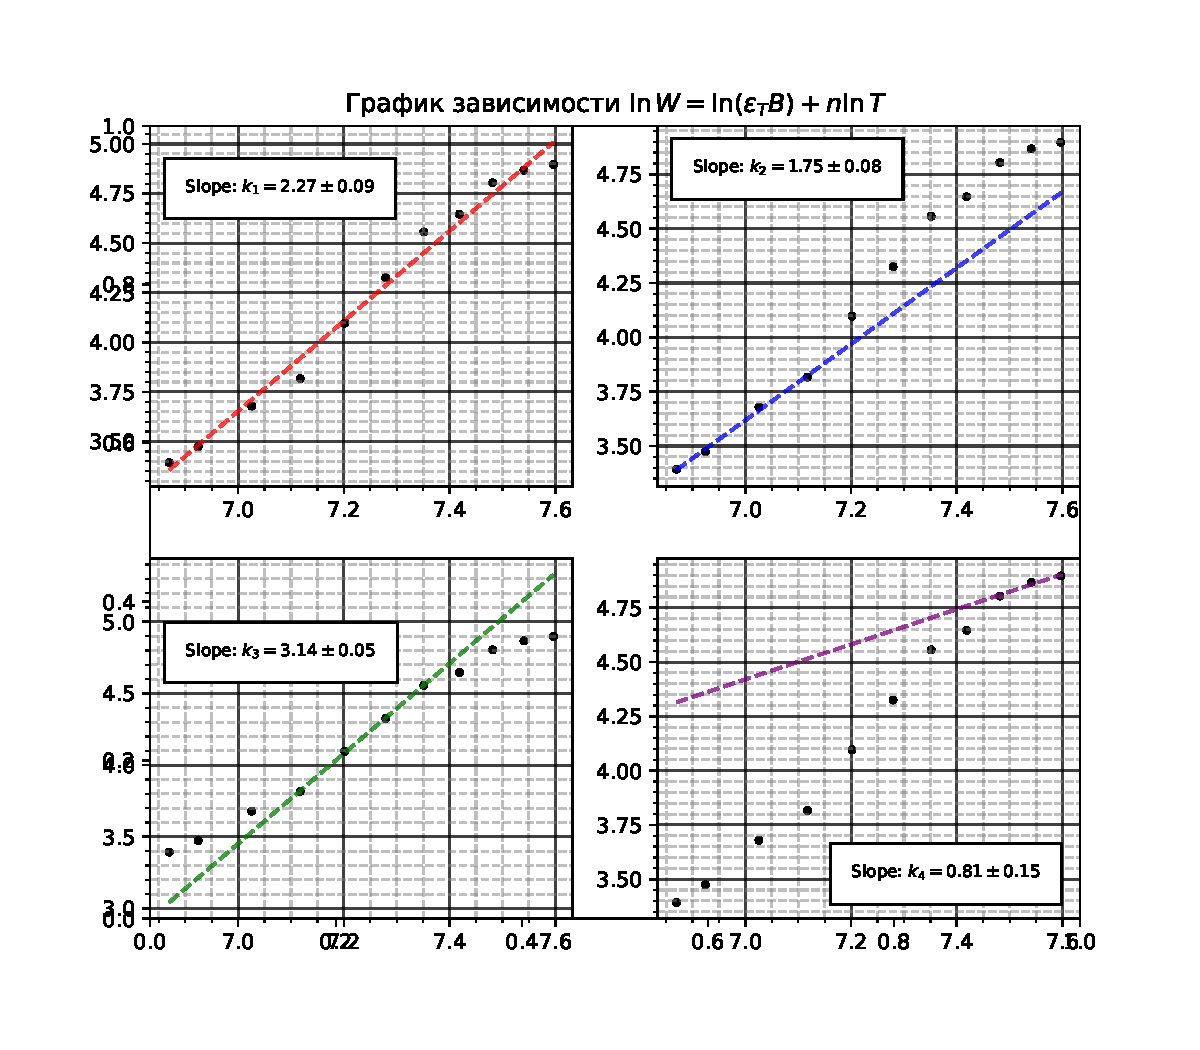
\includegraphics[width=\linewidth]{logW.pdf}
		% \caption{}
		\label{fig:logW}
	\end{figure}

	Как видно, наилучшее приближение к теоретическому значению $n = 4$ можно получить, если рассмастривать среднюю часть графика.

	Используя табличное значение $\varepsilon_T$ для вольфрама, найдем постоянную Стефана-Больцмана $\sigma$ 
	($B = S \sigma$, где $S = 0.36 \text{см}^2$ -- эффективная площадь излучающей поверхности нити). 

	\[\sigma = \frac{W}{\varepsilon_T S T^4} \]

	\begin{table}[h!]
    \begin{tabular}{|c|c|c|c|c|}
    \hline
    $T$, C       & $T$, K    & $\varepsilon_T$   & $W$, мВт      & $\sigma \cdot 10^{-9}$ \\ \hline
    962,50       & 1235,50   & 0,105             & 29,76         & 3,38                   \\ \hline
    1016,67      & 1289,67   & 0,105             & 32,25         & 3,08                   \\ \hline
    1125,00      & 1398,00   & 0,119             & 39,60         & 2,42                   \\ \hline
    1233,33      & 1506,33   & 0,133             & 45,46         & 1,84                   \\ \hline
    1341,67      & 1614,67   & 0,144             & 60,12         & 1,71                   \\ \hline
    1450,00      & 1723,00   & 0,164             & 75,58         & 1,45                   \\ \hline
    1558,33      & 1831,33   & 0,179             & 95,26         & 1,31                   \\ \hline
    1666,67      & 1939,67   & 0,195             & 104,22        & 1,05                   \\ \hline
    1775,00      & 2048,00   & 0,209             & 122,03        & 0,92                   \\ \hline
    \end{tabular}
    \centering
    \caption{}
    \label{tabel:calculations}
\end{table}

	\begin{center}
		\fbox{$\sigma = 1.9 \cdot 10^{-9} ~ \frac{\text{Вт}}{\text{см}^2 K^4}$}
	\end{center}

	По найденным значениям $\sigma$ посчитаем постоянную планка $h$, используя формулу

	\[ h = ^3\sqrt{\frac{2 \pi^5 k_{\text{Б}}^4}{15 c^2 \sigma}} \]

	\begin{center}
		\fbox{$h = 2.05 \cdot 10^{-33}$ Дж$\cdot$с}
	\end{center}

	\section*{Измерение <<яркостной температуры>> неоновой лампы}

	Термодинамическая температура неоновой лампочки примерно равна комнатной, и не соответствует её яркостной температуре ($\approx$ 820$^{\circ}$C). 
	Дело в том, что неоновая лампочка в принципе не является моделью абсолютно чёрного или серого тела, 
	и её излучение носит совершенно другую природу (переход электронов между энергетическими уровнями). 
	То, что её свет имеет такой же цвет, что и нагретое АЧТ - совпадение.
\end{document}